\documentclass[a4paper,12pt]{article}

\usepackage{cmap}          % поиск в PDF
\usepackage{mathtext}         % русские буквы в формулах
\usepackage[T2A]{fontenc}      % кодировка
\usepackage[utf8]{inputenc}      % кодировка исходного текста
\usepackage[english,russian]{babel}  % локализация и переносы
\usepackage[left=2cm,right=2cm,top=2cm,bottom=2cm]{geometry}
\usepackage{amsfonts,amssymb,amsthm,mathtools} % AMS
\usepackage{amsmath}
\usepackage{icomma} % "Умная" запятая: $0,2$ --- число, $0, 2$
\usepackage{graphicx}
\usepackage{wrapfig} % картинка в тектсе
\usepackage{caption} % убирается номер у подписей caption*{}
\usepackage{csquotes} % цитаты
\usepackage{multirow} % для жестких таблиц
\usepackage{hhline}
\usepackage{indentfirst} % абзацный отступ после section
\usepackage{epigraph} % эпиграф
\usepackage{tikz}
\usepackage{pgfplots}
\usepackage[export]{adjustbox}
\usepackage{tabularx}
\usepackage{float}
\usepackage{longtable}

\title{\textbf{Измерение коэффициента поверхностного натяжения жидкости. (2.5.1)}}
\author{Зайнуллин Амир Б05-206}

\begin{document}

\maketitle

\section{Аннотация}

\textbf{Цель работы:} 
1) измерение температурной зависимости  коэффициента поверхностного натяжения дистиллированной воды с использованием известного коэффициента поверхностного натяжения спирта; 2) определение полной поверхностной энергии  и теплоты, необходимой для изотермического образования единицы  поверхности жидкости  при различной температуре.
	
\textbf{В работе используются:} 
прибор  Ребиндера  с термостатом и микроманометром; исследуемые жидкости; стаканы; микроскоп.
	
\section{Теоретические сведения}
Из-за поверхностного натяжения возникают разные давления с разных сторон искривленной поверхности жидкости:
\begin{equation}
\Delta P = P_{внутри} - P_{снаружи} = \frac{2\sigma}{r} \;(формула\; Лапласа)
\end{equation}
$\sigma$ - коэффицент поверхностного натяжения, $r$ - радиус кривизны поверхности.

\section{Экспериментальная установка и методика измерений}

Тестовая жидкость (этиловый спирт) наливается в сосуд, через пробку в него входит полая металлическа игла. При создании достаточно разреженного воздуха в колбе пузырьки воздуха начинают пробулькивать, поверхностное натяжение измеряется по величине разряжения. Разряжение создается с помощью аспиратора, разность давлений измеряется спиртовым микроманометром.

Для стабилизации температуры через рубашку колбы с исследуемой жидкостью прогоняется вода из термостата. Из-за большой теплопроводности трубки температура в разных частях трубки заметно различна и ввиду теплового расширения поднимается уровень жидкости при изменении температуры. Поэтому при температурном измерениии кончик иглы опускают до самого дна сосуда, тогда:
\begin{equation}
\Delta P = P - \rho g h
\end{equation}
$\rho$ - плотность жидкости, $h$ - высота погружения иглы.

\begin{figure}[H]
    \begin{center}
    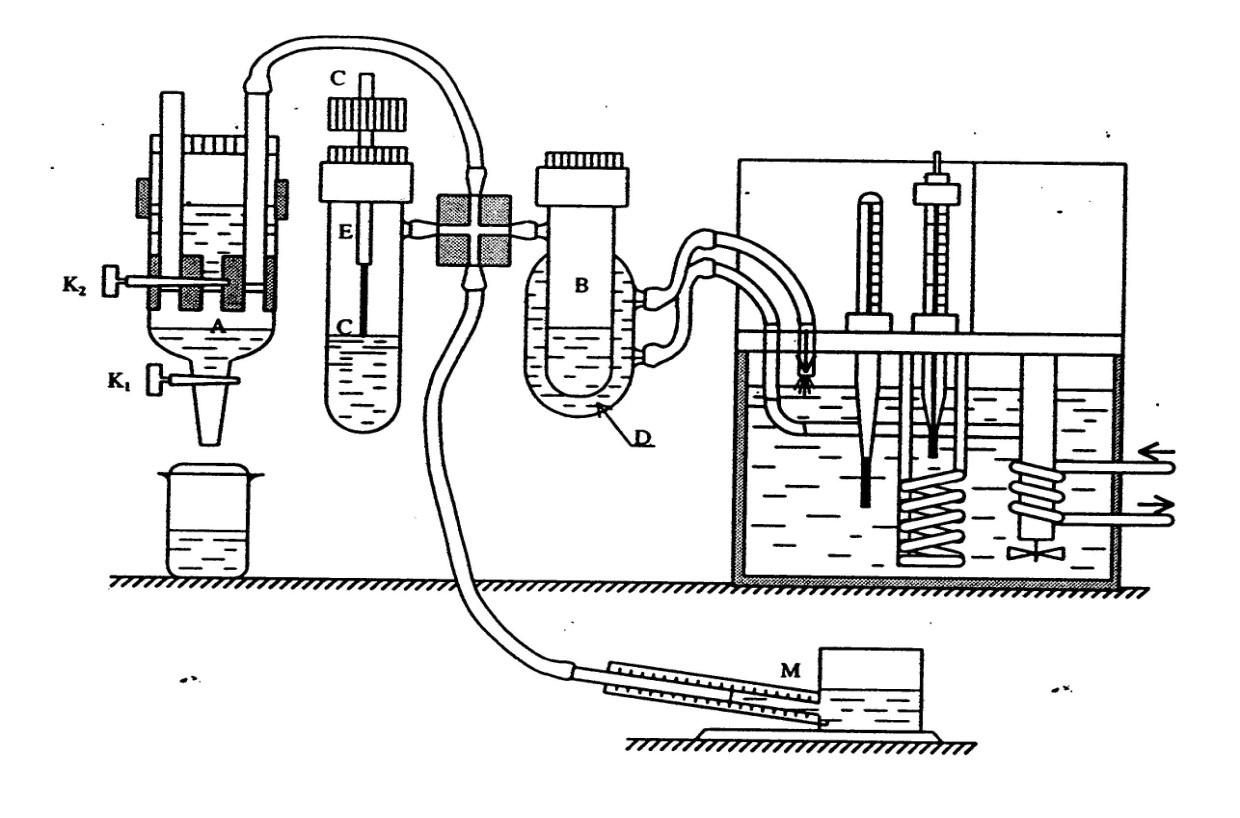
\includegraphics[width=0.8\textwidth]{Установка}
    \end{center}
    \caption{Схема установки}
\end{figure}

\subsection*{Методика измерений}
\begin{enumerate}
    \item Измерим диаметр иглы. 
    \item Определим поправку при измерении давления для погруженной в воду иглы. Утопим иглу до предела. Измерим h2. Измерьте максимальное давление в пузырьках. По разности давлений определим глубину погружения.
    \item Снимем температурную зависимость $\sigma (T)$ дистиллированной воды. Проводить измерение температурной зависимости рекомендуется в диапазоне 20 - 60 градусов. Для установления температуры жидкости будем ждать пару минут. 
\end{enumerate}

\section{Результаты измерений и обработка данных}

\subsection*{Измерение диаметра иглы}
Измерим максимальное давление при пробулькивании пузырьков воздуха через спирт. 

\begin{table}[H]
    \centering
    \begin{tabular}{|c|c|c|}
    \hline
        № & $P$, дел & $P$, Па  \\ \hline
        1 & 42 & 82,404 \\ \hline
        2 & 43 & 84,366 \\ \hline
        3 & 42 & 82,404 \\ \hline
        4 & 42 & 82,404 \\ \hline
        5 & 42 & 82,404 \\ \hline
    \end{tabular}
    \caption{Измерения в спирте}
\end{table}

\begin{table}[H]
    \centering
    \begin{tabular}{|c|c|c|c|c|}
    \hline
        $P_{ср}$, Па & $P_{сл}$, Па & $P_{сист}$, Па & $\sigma_P$, Па & $\varepsilon_P$ \\ \hline
        82,8 & 0,4 & 2,0 & 2,0 & 0,02 \\ \hline
    \end{tabular}
    \caption{Результаты}
\end{table}

По формуле найдем диаметр иглы:
	\begin{equation}
		d = \frac{4\sigma_{\text{с}}}{P_\text{макс}} = (1,10 \pm 0.03)\text{ мм}.
	\end{equation}
	
	Результат полученный под микроскопом: $D = (1,15\pm0.05)$ мм, это означает, что диаметр найденный экспериментально достаточно точен.
	
\subsection{Определения поправки при измерении давления для погруженной в воду иглы}

Перенесём предварительно промытую и просушенную от спирта иглу в колбу с дистиллированной водой. Измерим максимальное давление $ P_1 $ при пробулькивании пузырьков, когда игла лишь касается поверхности воды. Измерите расстояние между верхним концом иглы и любой неподвижной часть прибора $ h_1 $.

Утопим иглу в воду. Измерим $ h_2 $. Также измерим максимальное давление в пузырьках $ P_2 $. Полученные результаты заносим в таблицу.

\begin{table}[H]
    \centering
    \begin{tabular}{|c|c|c|}
    \hline
        № & дел & P, Па \\ \hline
        1 & 126 & 247,2 \\ \hline
        2 & 126 & 247,2 \\ \hline
        3 & 125 & 245,3 \\ \hline
        4 & 126 & 247,2 \\ \hline
        5 & 125 & 245,3 \\ \hline
        6 & 126 & 247,2 \\ \hline
    \end{tabular}
\end{table}

\begin{table}[H]
    \centering
    \begin{tabular}{|c|c|c|c|c|c|}
    \hline
        $P_{ср}$, Па & $\sigma_P^{случ}$, Па & $\sigma_P^{сист}$, Па & $\sigma_P$, Па & $\varepsilon_P$ & $h_1$, мм \\ \hline
        246,56 & 0,41 & 1,96 & 2,01 & 0,01 & 21 \\ \hline
    \end{tabular}
    \caption{Результаты измерений $P_1$}
\end{table}

\begin{table}[H]
    \centering
    \begin{tabular}{|c|c|c|}
    \hline
        № & дел & P, Па \\ \hline
        1 & 192 & 376,70 \\ \hline
        2 & 191 & 374,74 \\ \hline
        3 & 191 & 374,74 \\ \hline
        4 & 192 & 376,70 \\ \hline
        5 & 192 & 376,70 \\ \hline
        6 & 192 & 376,70 \\ \hline
    \end{tabular}
\end{table}

\begin{table}[H]
    \centering
    \begin{tabular}{|c|c|c|c|c|c|}
    \hline
        $P_{ср}$, Па & $\sigma_P^{случ}$, Па & $\sigma_P^{сист}$, Па & $\sigma_P$, Па & $\varepsilon_P$ & $h_1$, мм \\ \hline
        376,05 & 0,41 & 1,96 & 2,01 & 0,01 & 8 \\ \hline
    \end{tabular}
    \caption{Результаты измерений $P_2$}
\end{table}


Также вычисляем погрешность:  \begin{equation}
	\sigma_{\Delta P} = \sqrt{\sigma^2_{P_1}+\sigma^2_{P_2}} \approx 2,8 \text{ Па}.
\end{equation}

Таким образом, получаем 
\begin{equation}
    \Delta P = (129,5 \pm 2,8) \text{ Па}
\end{equation}

По полученному значению $ \Delta P $ можем рассчитать $ \Delta h $ по следующей формуле: \[ \Delta h = \frac{\Delta P}{\rho g} \approx 13,2 \text{ мм}, \] где $ \rho = 1000 $ кг/$ \text{м}^3 $ -- плотность воды и $ g = 9,81 $ м/$ \text{с}^2 $ -- ускорение свободного падения.

\medskip

При этом погрешность нашего измерения равна \[ \sigma_{\Delta h} = \Delta h \cdot \varepsilon_{\Delta P} \approx 0,3 \text{ мм}. \]

Таким образом, получаем $\Delta h = (13,2 \pm 0,3) \text{ мм} $

\medskip

Заметим, что полученный результат в пределах погрешности совпадает с результатом, полученном прямым измерением $\Delta h' = (13 \pm 0,71) \text{ мм}. $

Значит, в ходе дальнейших измерений мы будем делать поправку $ \Delta P = (129,5 \pm 2,8) \text{ Па} $ на добавочное давление со стороны столба жидкости.



\subsection*{Измерение температурной зависимости коэффициента поверхностного натяжения}

Снимем температурную зависимость $ \sigma(T) $ дистиллированной воды. Для этого включим термостат и подождём, пока нужная нам температура не стабилизируется. После этого проведём измерение давления. Для уменьшения погрешности опыта замер давления  при фиксированной температуре проведём несколько раз. Результаты измерений занесём в таблицу

\begin{table}[H]
\begin{tabular}{|c|c|c|c|c|c|c|c|c|c|}
\hline
\multicolumn{1}{|l|}{$ T $, К} & $ P' $, дел & $ P' $, Па & \multicolumn{1}{l|}{$ \langle P' \rangle $, Па} & \multicolumn{1}{l|}{$\sigma_P^{случ}$, Па} & \multicolumn{1}{l|}{$\sigma_P^{сист}$, Па} & \multicolumn{1}{l|}{$ \sigma_{P'} $, Па} & \multicolumn{1}{l|}{$ P $, Па} & \multicolumn{1}{l|}{$ \sigma_P $, Па} & \multicolumn{1}{l|}{$\varepsilon_P$} \\ \hline
\multirow{5}{*}{298}           & 192         & 376,7      & \multirow{5}{*}{377,1}                          & \multirow{5}{*}{0,4}                       & \multirow{5}{*}{2,0}                       & \multirow{5}{*}{2,0}                     & \multirow{5}{*}{247,6}         & \multirow{5}{*}{3,4}                  & \multirow{5}{*}{0,01}                \\ \cline{2-3}
                               & 192         & 376,7      &                                                 &                                            &                                            &                                          &                                &                                       &                                      \\ \cline{2-3}
                               & 193         & 378,7      &                                                 &                                            &                                            &                                          &                                &                                       &                                      \\ \cline{2-3}
                               & 192         & 376,7      &                                                 &                                            &                                            &                                          &                                &                                       &                                      \\ \cline{2-3}
                               & 192         & 376,7      &                                                 &                                            &                                            &                                          &                                &                                       &                                      \\ \hline
\end{tabular}
\end{table}


\begin{table}[H]
\begin{tabular}{|c|c|c|c|c|c|c|c|c|c|}
\hline
\multicolumn{1}{|l|}{$ T $, К} & $ P' $, дел & $ P' $, Па & \multicolumn{1}{l|}{$ \langle P' \rangle $, Па} & \multicolumn{1}{l|}{$\sigma_P^{случ}$, Па} & \multicolumn{1}{l|}{$\sigma_P^{сист}$, Па} & \multicolumn{1}{l|}{$ \sigma_{P'} $, Па} & \multicolumn{1}{l|}{$ P $, Па} & \multicolumn{1}{l|}{$ \sigma_P $, Па} & \multicolumn{1}{l|}{$\varepsilon_P$} \\ \hline
\multirow{5}{*}{303}           & 192         & 376,7      & \multirow{5}{*}{376,7}                          & \multirow{5}{*}{0,0}                       & \multirow{5}{*}{2,0}                       & \multirow{5}{*}{2,0}                     & \multirow{5}{*}{247,2}         & \multirow{5}{*}{3,4}                  & \multirow{5}{*}{0,01}                \\ \cline{2-3}
                               & 192         & 376,7      &                                                 &                                            &                                            &                                          &                                &                                       &                                      \\ \cline{2-3}
                               & 192         & 376,7      &                                                 &                                            &                                            &                                          &                                &                                       &                                      \\ \cline{2-3}
                               & 192         & 376,7      &                                                 &                                            &                                            &                                          &                                &                                       &                                      \\ \cline{2-3}
                               & 192         & 376,7      &                                                 &                                            &                                            &                                          &                                &                                       &                                      \\ \hline
\end{tabular}
\end{table}


\begin{table}[H]
\begin{tabular}{|c|c|c|c|c|c|c|c|c|c|}
\hline
\multicolumn{1}{|l|}{$ T $, К} & $ P' $, дел & $ P' $, Па & \multicolumn{1}{l|}{$ \langle P' \rangle $, Па} & \multicolumn{1}{l|}{$\sigma_P^{случ}$, Па} & \multicolumn{1}{l|}{$\sigma_P^{сист}$, Па} & \multicolumn{1}{l|}{$ \sigma_{P'} $, Па} & \multicolumn{1}{l|}{$ P $, Па} & \multicolumn{1}{l|}{$ \sigma_P $, Па} & \multicolumn{1}{l|}{$\varepsilon_P$} \\ \hline
\multirow{5}{*}{308}           & 191         & 374,7      & \multirow{5}{*}{373,2}                          & \multirow{5}{*}{0,4}                       & \multirow{5}{*}{2,0}                       & \multirow{5}{*}{2,0}                     & \multirow{5}{*}{243,7}         & \multirow{5}{*}{3,4}                  & \multirow{5}{*}{0,01}                \\ \cline{2-3}
                               & 190         & 372,8      &                                                 &                                            &                                            &                                          &                                &                                       &                                      \\ \cline{2-3}
                               & 190         & 372,8      &                                                 &                                            &                                            &                                          &                                &                                       &                                      \\ \cline{2-3}
                               & 190         & 372,8      &                                                 &                                            &                                            &                                          &                                &                                       &                                      \\ \cline{2-3}
                               & 190         & 372,8      &                                                 &                                            &                                            &                                          &                                &                                       &                                      \\ \hline
\end{tabular}
\end{table}


\begin{table}[H]
\begin{tabular}{|c|c|c|c|c|c|c|c|c|c|}
\hline
\multicolumn{1}{|l|}{$ T $, К} & $ P' $, дел & $ P' $, Па & \multicolumn{1}{l|}{$ \langle P' \rangle $, Па} & \multicolumn{1}{l|}{$\sigma_P^{случ}$, Па} & \multicolumn{1}{l|}{$\sigma_P^{сист}$, Па} & \multicolumn{1}{l|}{$ \sigma_{P'} $, Па} & \multicolumn{1}{l|}{$ P $, Па} & \multicolumn{1}{l|}{$ \sigma_P $, Па} & \multicolumn{1}{l|}{$\varepsilon_P$} \\ \hline
\multirow{5}{*}{313}           & 189         & 370,8      & \multirow{5}{*}{370,4}                          & \multirow{5}{*}{0,4}                       & \multirow{5}{*}{2,0}                       & \multirow{5}{*}{2,0}                     & \multirow{5}{*}{240,9}         & \multirow{5}{*}{3,4}                  & \multirow{5}{*}{0,01}                \\ \cline{2-3}
                               & 189         & 370,8      &                                                 &                                            &                                            &                                          &                                &                                       &                                      \\ \cline{2-3}
                               & 188         & 368,9      &                                                 &                                            &                                            &                                          &                                &                                       &                                      \\ \cline{2-3}
                               & 189         & 370,8      &                                                 &                                            &                                            &                                          &                                &                                       &                                      \\ \cline{2-3}
                               & 189         & 370,8      &                                                 &                                            &                                            &                                          &                                &                                       &                                      \\ \hline
\end{tabular}
\end{table}


\begin{table}[H]
\begin{tabular}{|c|c|c|c|c|c|c|c|c|c|}
\hline
\multicolumn{1}{|l|}{$ T $, К} & $ P' $, дел & $ P' $, Па & \multicolumn{1}{l|}{$ \langle P' \rangle $, Па} & \multicolumn{1}{l|}{$\sigma_P^{случ}$, Па} & \multicolumn{1}{l|}{$\sigma_P^{сист}$, Па} & \multicolumn{1}{l|}{$ \sigma_{P'} $, Па} & \multicolumn{1}{l|}{$ P $, Па} & \multicolumn{1}{l|}{$ \sigma_P $, Па} & \multicolumn{1}{l|}{$\varepsilon_P$} \\ \hline
\multirow{5}{*}{318}           & 187         & 366,9      & \multirow{5}{*}{367,7}                          & \multirow{5}{*}{0,5}                       & \multirow{5}{*}{2,0}                       & \multirow{5}{*}{2,0}                     & \multirow{5}{*}{238,2}         & \multirow{5}{*}{3,5}                  & \multirow{5}{*}{0,01}                \\ \cline{2-3}
                               & 187         & 366,9      &                                                 &                                            &                                            &                                          &                                &                                       &                                      \\ \cline{2-3}
                               & 188         & 368,9      &                                                 &                                            &                                            &                                          &                                &                                       &                                      \\ \cline{2-3}
                               & 187         & 366,9      &                                                 &                                            &                                            &                                          &                                &                                       &                                      \\ \cline{2-3}
                               & 188         & 368,9      &                                                 &                                            &                                            &                                          &                                &                                       &                                      \\ \hline
\end{tabular}
\end{table}

\begin{table}[H]
\begin{tabular}{|c|c|c|c|c|c|c|c|c|c|}
\hline
\multicolumn{1}{|l|}{$ T $, К} & $ P' $, дел & $ P' $, Па & \multicolumn{1}{l|}{$ \langle P' \rangle $, Па} & \multicolumn{1}{l|}{$\sigma_P^{случ}$, Па} & \multicolumn{1}{l|}{$\sigma_P^{сист}$, Па} & \multicolumn{1}{l|}{$ \sigma_{P'} $, Па} & \multicolumn{1}{l|}{$ P $, Па} & \multicolumn{1}{l|}{$ \sigma_P $, Па} & \multicolumn{1}{l|}{$\varepsilon_P$} \\ \hline
\multirow{5}{*}{323}           & 186         & 364,9      & \multirow{5}{*}{365,3}                          & \multirow{5}{*}{0,4}                       & \multirow{5}{*}{2,0}                       & \multirow{5}{*}{2,0}                     & \multirow{5}{*}{235,8}         & \multirow{5}{*}{3,4}                  & \multirow{5}{*}{0,01}                 \\ \cline{2-3}
                               & 186         & 364,9      &                                                 &                                            &                                            &                                          &                                &                                       &                                      \\ \cline{2-3}
                               & 186         & 364,9      &                                                 &                                            &                                            &                                          &                                &                                       &                                      \\ \cline{2-3}
                               & 187         & 366,9      &                                                 &                                            &                                            &                                          &                                &                                       &                                      \\ \cline{2-3}
                               & 186         & 364,9      &                                                 &                                            &                                            &                                          &                                &                                       &                                      \\ \hline
\end{tabular}
\end{table}

\begin{table}[H]
\begin{tabular}{|c|c|c|c|c|c|c|c|c|c|}
\hline
\multicolumn{1}{|l|}{$ T $, К} & $ P' $, дел & $ P' $, Па & \multicolumn{1}{l|}{$ \langle P' \rangle $, Па} & \multicolumn{1}{l|}{$\sigma_P^{случ}$, Па} & \multicolumn{1}{l|}{$\sigma_P^{сист}$, Па} & \multicolumn{1}{l|}{$ \sigma_{P'} $, Па} & \multicolumn{1}{l|}{$ P $, Па} & \multicolumn{1}{l|}{$ \sigma_P $, Па} & \multicolumn{1}{l|}{$\varepsilon_P$} \\ \hline
\multirow{5}{*}{328}           & 185         & 363,0      & \multirow{5}{*}{362,6}                          & \multirow{5}{*}{0,4}                       & \multirow{5}{*}{2,0}                       & \multirow{5}{*}{2,0}                     & \multirow{5}{*}{233,1}         & \multirow{5}{*}{3,4}                  & \multirow{5}{*}{0,01}                \\ \cline{2-3}
                               & 185         & 363,0      &                                                 &                                            &                                            &                                          &                                &                                       &                                      \\ \cline{2-3}
                               & 185         & 363,0      &                                                 &                                            &                                            &                                          &                                &                                       &                                      \\ \cline{2-3}
                               & 184         & 361,0      &                                                 &                                            &                                            &                                          &                                &                                       &                                      \\ \cline{2-3}
                               & 185         & 363,0      &                                                 &                                            &                                            &                                          &                                &                                       &                                      \\ \hline
\end{tabular}
\end{table}

\begin{table}[H]
\begin{tabular}{|c|c|c|c|c|c|c|c|c|c|}
\hline
\multicolumn{1}{|l|}{$ T $, К} & $ P' $, дел & $ P' $, Па & \multicolumn{1}{l|}{$ \langle P' \rangle $, Па} & \multicolumn{1}{l|}{$\sigma_P^{случ}$, Па} & \multicolumn{1}{l|}{$\sigma_P^{сист}$, Па} & \multicolumn{1}{l|}{$ \sigma_{P'} $, Па} & \multicolumn{1}{l|}{$ P $, Па} & \multicolumn{1}{l|}{$ \sigma_P $, Па} & \multicolumn{1}{l|}{$\varepsilon_P$} \\ \hline
\multirow{5}{*}{333}           & 184         & 361,0      & \multirow{5}{*}{360,2}                          & \multirow{5}{*}{0,5}                       & \multirow{5}{*}{2,0}                       & \multirow{5}{*}{2,0}                     & \multirow{5}{*}{230,7}         & \multirow{5}{*}{3,5}                  & \multirow{5}{*}{0,01}                \\ \cline{2-3}
                               & 183         & 359,0      &                                                 &                                            &                                            &                                          &                                &                                       &                                      \\ \cline{2-3}
                               & 184         & 361,0      &                                                 &                                            &                                            &                                          &                                &                                       &                                      \\ \cline{2-3}
                               & 184         & 361,0      &                                                 &                                            &                                            &                                          &                                &                                       &                                      \\ \cline{2-3}
                               & 183         & 359,0      &                                                 &                                            &                                            &                                          &                                &                                       &                                      \\ \hline
\end{tabular}
\caption{Результаты измерений}
\end{table}


Также учитываем поправку к измеренному давлению, которая была вычислена в формуле (5). Полученные результаты также заносим в таблицу.

По полученным данным вычислим коэффициент поверхностного натяжения для каждой из температур по формуле

\begin{equation}
	\sigma = \frac{Pd}{4},
\end{equation}
где $ d $ -- диаметр иглы. Погрешность такого результата вычисляется по следующей формуле:

\begin{equation}
	\sigma_\sigma = \sigma\sqrt{\varepsilon^2_P + \varepsilon^2_d}.
\end{equation}

Полученные результаты заносим в таблицу.

\begin{table}[H]
    \centering
    \begin{tabular}{|c|c|c|c|c|}
    \hline
        № & $ T $, К   & $ \sigma_T, К $   & $ \sigma $, мН/м & $ \sigma_\sigma $, мН/м \\ \hline
        1 & 298,0 & 0,2 & 68,1 & 1,8 \\ \hline
        2 & 303,0 & 0,2 & 68,0 & 1,8 \\ \hline
        3 & 308,0 & 0,2 & 67,0 & 1,7 \\ \hline
        4 & 313,0 & 0,2 & 66,3 & 1,7 \\ \hline
        5 & 318,0 & 0,2 & 65,5 & 1,7 \\ \hline
        6 & 323,0 & 0,2 & 64,9 & 1,7 \\ \hline
        7 & 328,0 & 0,2 & 64,1 & 1,7 \\ \hline
    \end{tabular}
    \caption{Полученные результаты вычислений}
\end{table}

Строим на графике полученную зависимость и считаем коэффицент наклона графика по МНК. 

\begin{figure}[H]
    \begin{center}
    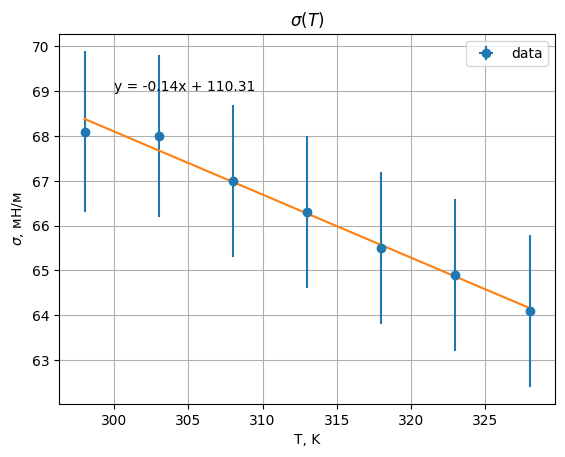
\includegraphics[width=0.7\textwidth]{sigmaT.png}
    \end{center}
    \caption{Зависимость $\sigma (T)$}
\end{figure}

\[ k = \frac{d\sigma}{dT} = (-0,140 \pm 0,007) \text{ } \frac{\text{мН}}{\text{м}\cdot\text{К}} \]
Построим также зависимость теплоты образования единицы поверхности жидкости от температуры $q(T) = -T \frac{d\sigma}{dT}$ и поверхностной энергии единицы площади от температуры $\frac{U}{F} = \left(\sigma - T \frac{d\sigma}{dT}\right)$

\begin{table}[H]
    \centering
    \begin{tabular}{|c|c|c|c|c|c|}
    \hline
        № & $ T $, К & $q$, мН/м & $\sigma_q$ мН/м & $\frac{U}{F}$, мН/м & $\sigma_{\frac{U}{F}}$,  мН/м\\ \hline
        1 & 298 & 41,7 & 2,1 & 109,8 & 3,8 \\ \hline
        2 & 303 & 42,4 & 2,1 & 110,4 & 3,9 \\ \hline
        3 & 308 & 43,1 & 2,2 & 110,1 & 3,9 \\ \hline
        4 & 313 & 43,8 & 2,2 & 110,1 & 3,9 \\ \hline
        5 & 318 & 44,5 & 2,2 & 110,0 & 3,9 \\ \hline
        6 & 323 & 45,2 & 2,3 & 110,1 & 4,0 \\ \hline
        7 & 328 & 45,9 & 2,3 & 110,0 & 4,0 \\ \hline
    \end{tabular}
    \caption{Данные для графиков}
\end{table}

\begin{figure}[H]
    \begin{center}
    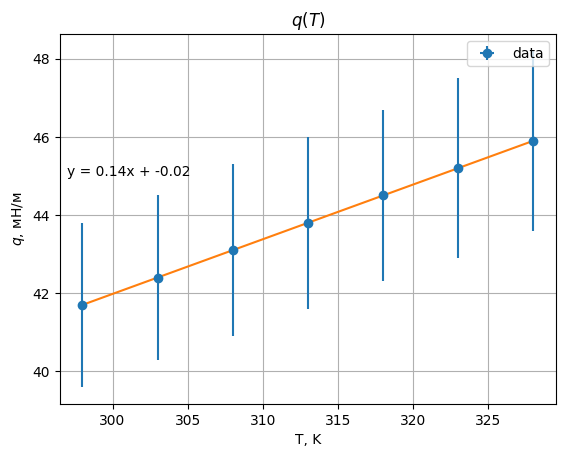
\includegraphics[width=0.65\textwidth]{q(T).png}
    \end{center}
\end{figure}

\begin{figure}[H]
    \begin{center}
    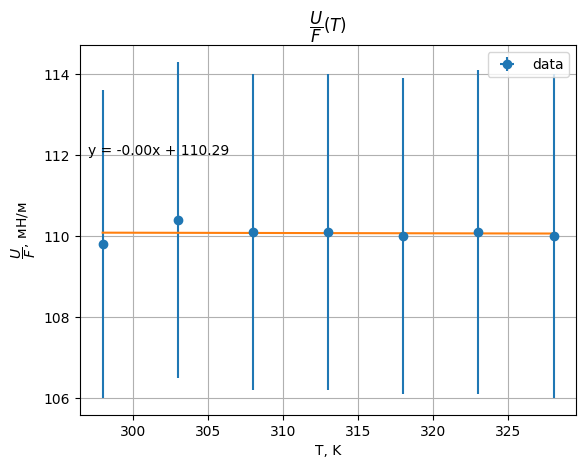
\includegraphics[width=0.65\textwidth]{U:F.png}
    \end{center}
\end{figure}

\section{Выводы}

\begin{enumerate}
    \item В ходе работы был измерен диаметр иглы двумя способами. Первый способ - при помощи известного коэффициента поверхностного натяжения спирта. Полученный результат сходится с хорошей точностью со вторым cпособом - измерением диаметра микроскопом.
    \item Было определено добавочное давление, создаваемое жидкостью при опускании иглы на некоторую высоту. Данная величина так же сходится с прямым измерением высоты. Полученная поправка была использована в основной части работы. Игла была погружена в основной части работы для увеличения точности измерений.
    \item Был экспериментально получен коэффицент поверхностного натяжения воды для 7 различных температур в диапазоне 25-60 градусов. Мы выяснили, что коэффицент поверхностного натяжения зависит от температуры прямо пропорционально. Данные хорошо ложились на линейную зависимость, несмотря на большие кресты погрешности. 
    \item Табличное значение коэффициента поверхностного натяжения дистиллированной воды при 20 градусах равен 72 мН/м. Что почти сходится с нашим полученным результатом. Значит данная лабораторная работа обладает хорошей точностью. 
    \item Полученные результаты дают основание полагать, что теоретические данные довольно точно описывают наблюдаемые зависимости. 
    \item С помощью графиков убедились, что зависимость теплоты образования единицы поверхности жидкости от температуры линейна. А поверхностная энергия единицы площади от температуры \textbf{не зависит}. 

\end{enumerate}




\end{document}